\documentclass[UTF8,ctexart,a4paper,11pt,openany]{article}
\usepackage[slantfont,boldfont]{xeCJK}
\usepackage{fontspec}
\usepackage{ctex}

\setCJKmainfont{SimSun}%[BoldFont=SimHei] %去掉注释:bf字体为黑体

\setsansfont{SimHei}
\setCJKsansfont{SimHei}

\xeCJKsetcharclass{"2160}{"2470}{1}% 1: CJK
\xeCJKsetup{AutoFallBack=true}
\setCJKfallbackfamilyfont{\CJKrmdefault}{SimSun.ttf}

%\setmainfont{Times New Roman}     %去掉注释:Times new roman字体
%\usepackage{mathptmx}             %去掉注释:Times new roman字体

\usepackage{mathtools}
\usepackage{amsmath}
\usepackage{amsfonts}
\usepackage{amssymb}
\usepackage{amsthm}
\usepackage[T1]{fontenc}
\usepackage{indentfirst} %段首空两格

\usepackage{graphicx}
\usepackage{geometry}
\usepackage{latexsym}
\usepackage{fancyhdr}
\usepackage{epstopdf}
%\usepackage{pifont}
%\usepackage[perpage,symbol*]{footmisc}
\usepackage{titlesec}
\usepackage{setspace}
\usepackage{enumerate}
\usepackage{enumitem}
\usepackage{multicol}
\usepackage{url}
\usepackage{exscale}
\usepackage{ulem}
\usepackage{relsize}
\usepackage{mathrsfs}
\usepackage{tikz}
\usepackage{wrapfig}
\usepackage{framed}
\usepackage{bm}
%\usepackage{pstricks,pst-node,multido,ifthen,calc}
\usepackage[all]{xy}
\usepackage{extarrows}
%\usepackage[backref]{hyperref}
\usepackage{hyperref}
\usepackage{stfloats} %插图的时候不分页

\setlength{\parindent}{2em} %段首空两格
\linespread{1.2}
\usepackage{listings}
\usepackage{xcolor}
\usepackage{algorithm}
\usepackage{algorithmicx}
\usepackage{algpseudocode}
\usepackage{mdframed}
\usepackage{extarrows}
\usepackage{diagbox}
\usepackage{makecell}

\theoremstyle{definition}
\mdfdefinestyle{theoremstyle}{%
linecolor=green!40,linewidth=.5pt,%
backgroundcolor=green!10,
skipabove=8pt,
skipbelow=5pt,
innerleftmargin=7pt,
innerrightmargin=7pt,
frametitlerule=true,%
frametitlerulewidth=.5pt,
frametitlebackgroundcolor=green!35,
frametitleaboveskip=0pt,
frametitlebelowskip=0pt,
innertopmargin=.4\baselineskip,
innerbottommargin=.4\baselineskip,
shadow=true,shadowsize=3pt,shadowcolor=black!20,
%theoremseparator={\hspace{1pt}},
theoremseparator={.},
nobreak=true,
}


\everymath{\displaystyle}

\newtheorem{definition}{\hspace{2em}定义}[section]
\newtheorem{axiom}{\hspace{2em}公理}

\mdtheorem[style=theoremstyle]{theorem}{定理}
\mdtheorem[style=theoremstyle]{example}{例}
\mdtheorem[style=theoremstyle]{exercise}{问题}
\newtheorem{lemma}[theorem]{\hspace{2em}引理}
\newtheorem{corollary}[theorem]{\hspace{2em}推论}

\newcommand*{\QED}{\hfill\ensuremath{\square}}
\newcommand*{\rmk}{\textbf{注:}}
\renewcommand*{\proof}{\textbf{证明:}}
\newcommand*{\tips}{\textbf{提示:}}
\newcommand*{\hard}{\textbf{\color{red}(难)}}
\newcommand*{\eqsmall}{\setlength\abovedisplayskip{1pt}\setlength\belowdisplayskip{1pt}}
\geometry{left=2cm,right=2cm,top=2cm,bottom=2cm}
% \title{数值分析上机报告(示例}
% \author{Fiddie}
\pagestyle{fancy}
\fancyfoot[C]{}
\fancyhead[RO]{ \thepage}
\fancyhead[LE]{\thepage  }
% \fancyhead[RE]{\rightmark (By Fiddie)}
% \fancyhead[LO]{\leftmark (By Fiddie)}
\titleformat{\chapter}{\centering\huge\bfseries}{第\,\thechapter\,章}{1em}{} %更改标题样式
\titleformat{\section}{\bfseries\Large}{$\S$\,\thesection\,}{1em}{} %更改标题样式
\titlespacing*{\chapter}{0pt}{9pt}{0pt} %调整标题间距
\setenumerate[1]{itemsep=0pt,partopsep=0pt,parsep=\parskip,topsep=0pt} %设置enumerate行间距
\setenumerate[2]{itemsep=0pt,partopsep=0pt,parsep=\parskip,topsep=0pt} %设置enumerate行间距
\setitemize[1]{itemsep=0pt,partopsep=0pt,parsep=\parskip,topsep=0pt} % 设置itemize行间距
\setlist[enumerate,2]{label=(\arabic*),topsep=0mm,itemsep=0mm,partopsep=0mm,parsep=\parskip}
    % 设置二层枚举为(1)样式
    
\newfontfamily\hei{SimHei}
\newcommand\textcf[1]{\textbf{\textsf{\hei{#1}}}}

\newcommand\e{\leftarrow}
%\renewcommand{\bibname}{参考文献}

\begin{document}
\begin{center}
{\huge \textbf{数值分析第1次上机作业}}

{\large 学号:221840189,姓名:王晨光}
\end{center}

\section{问题一}
    \subsection{问题}
    编程以二进制的形式显示单精度或双精度浮点数.
    \subsection{算法思路}
    二进制形式的单双精度浮点数表示分为三部分:符号位,指数,尾数. 通过它们的定义,我们可以逐个确定下来. 其中单精度浮点数通过一共32位二进制数表示,计算指数部分时偏置为127;双精度浮点数通过一共64位浮点数表示,计算指数部分时偏置为1023.
    \begin{algorithm}
        \caption{浮点数的二进制表示}
        \begin{algorithmic}[1] %每行显示行号
            \Require 一个十进制浮点数$a$.
            \Ensure 浮点数的单精度与双精度的二进制表示字符串$s_1$,$s_2$,或失败(超界)信息.
            \Function {Transform}{$a$}
                \If {$a$超出单精度范围}
                    \State 输出“超出单精度范围”
                \Else
                    \State $float \qquad a_1\e a$
                    \If {$a_1<0$}
                        \State 符号位为1,$a_1=|a_1|$
                    \Else 
                        \State 符号位为0
                    \EndIf
                    \State 分离$a_1$的整数部分$\bar{a_1}$与小数部分$a_1-\bar{a_1}$
                    \State 转换$\bar{a_1}$,$a_1-\bar{a_1}$为二进制
                    \State 指数部分为$length(\bar{a_1})-1+127$的二进制表示
                    \State 尾数部分为$\bar{a_1}$去掉首位后与$a_1-\bar{a_1}$合并
                    \State 按顺序输出符号位,指数,尾数,得到二进制表示的单精度浮点数
                \EndIf
                \If {$a$超出双精度范围}
                    \State 输出“超出双精度范围”
                \Else
                    \State $double \qquad a_2\e a$
                    \If {$a_1<0$}
                        \State 符号位为1,$a_2=|a_2|$
                    \Else 
                        \State 符号位为0
                    \EndIf
                    \State 分离$a_2$的整数部分$\bar{a_2}$与小数部分$a_2-\bar{a_2}$
                    \State 转换$\bar{a_2}$,$a_2-\bar{a_2}$为二进制
                    \State 指数部分为$length(\bar{a_2})-1+1023$的二进制表示
                    \State 尾数部分为$\bar{a_2}$去掉首位后与$a_2-\bar{a_2}$合并
                    \State 按顺序输出符号位,指数,尾数,得到二进制表示的双精度浮点数
                \EndIf
            \EndFunction
        \end{algorithmic}
    \end{algorithm}
    \subsection{结果分析}%重点(误差图、结果图、分析算法的收敛性(速度)、内存使用(时间、空间)、计算量、稳定性
    测试程序,得到123.456的单精度浮点数二进制表示为:\par 01000010 11110110 11101001 01111001 \par 双精度为:\par 01000000 01011110 11011101 00101111 00011010 10011111 10111110 01110111 \par
    经检验,结果正确无误.
    
\section{问题二} 
    \subsection{问题}
    编程找出单精度或双精度浮点数的机器精度、下溢值和上溢值并与理论值比较。(非规格化浮点数)
    \subsection{算法思路}
    以单精度浮点数为例,双精度浮点数同理.\par
    1. 机器精度\par
    在计算机浮点系统中,一个浮点数的表达形式是 $fl(x)=x(1+\varepsilon),\left|\varepsilon\right| \leqslant \varepsilon_{mach}$,其中$\varepsilon_{mach}$是机器精度,它说明了用浮点系统表示一个非零实数$x$的最大可能相对误差,即$|(fl(x)-x)/x \leqslant\varepsilon_{mach}|$.因此,我们可以令$a=1$,并不断除以$2$,直至$a$的大小在浮点系统中忽略不计,即与$x$相加后在计算机中判定为$x$,从而得到所需的机器精度.
    \begin{algorithm}
        \caption{计算机器精度}
        \begin{algorithmic}[1]
            \State $float \qquad a=1$
            \While  {$1+a/2\ne 1$} 
                \State $a \e a/2$
            \EndWhile
            \State 得到机器精度$a$
        \end{algorithmic}
    \end{algorithm}
    \par
    2. 上溢值 \par
    上溢值是计算机中对应类型所能储存的最大数,考虑数字在计算机中的二进制储存形式,我们假设一个float类型的数$a$,令$a=1$,从而我们可以将$a$乘以2,并逐次判断$a$是否仍等于$2\cdot a-a$,直至不满足循环条件时,即得上溢值.
    \begin{algorithm}
        \caption{计算上溢值}
        \begin{algorithmic}[1]
            \State $float \qquad a=1$
            \While {$a=2\cdot a-a$} 
            \State $a \e 2\cdot a$
            \EndWhile
            \State 得到上溢值$a$
        \end{algorithmic}
    \end{algorithm}
    \par
    3. 下溢值\par
    下溢值是计算机所能储存的最小非零正数,考虑到数据在计算机中的二进制保存形式,我们可以将数字1不断除以2,并逐次判断$a$是否等于0,从而至循环结束后可得下溢值.
    \begin{algorithm}[H]
        \caption{计算下溢值}
        \begin{algorithmic}[1]
            \State $float \qquad a=1$
            \While {$a/2\ne 0$} 
            \State $a \e a/2$
            \EndWhile
            \State 得到下溢值$a$
        \end{algorithmic}
    \end{algorithm}
    \subsection{结果分析}
    \begin{figure}[htbp]
        \centering
        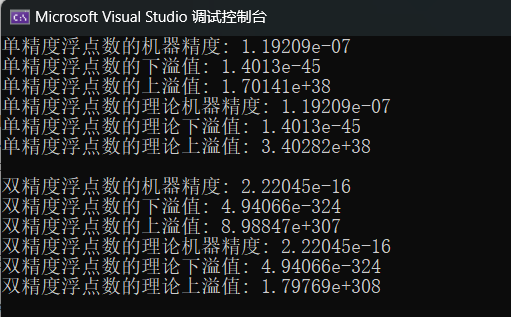
\includegraphics{pics/P2.1.png}
        \caption{问题二的算法最终结果与理论值对比}
        \label{graph:1}
        \end{figure}
    1.我们调用limits库中的numeric\_limits<float>::epsilon()从而得到单精度浮点数所储存的理论机器精度:1.19209e-07, 这与我们所写程序得到的结果一致,从而证明该方法一定程度上是正确的,我们求出了单精度浮点数的机器精度.\par 
    \vspace{10pt}
    2.我们调用limits库中的numeric\_limits<float>::max()从而得到单精度浮点数所储存的理论上溢值:3.40282e+38, 而程序所得结果为1.70141e+38,基本可以认定为理论值的$1/2$,可能是循环过程中累计的机器误差导致在最后一次循环后结果偏大,无法通过判断语句,从而影响最终结果. 根据单精度浮点数的结构,若让单精度浮点数可取得最大正值,可以令指数位为127(根据程序所得结果,该值与现实中一致),再令尾数位均取得1,即$(2-2^{-23})\times2^{127}=3.40282\times10^{38}$. 这与limits库中存储的理论上溢值一致. \par 
    \vspace{10pt}
    3.我们调用limits库中的numeric\_limits<float>::denorm\_min()从而得到单精度浮点数所储存的理论下溢值:1.4013e-45, 这与我们所写程序得到的结果一致,从而证明该方法一定程度上是正确的,我们求出了单精度浮点数的下溢值. \par
\section{结论}
根据单双精度浮点数的二进制表示的定义,可以得到将十进制数转换为二进制浮点数的算法. \par

单精度浮点数的机器精度为:1.19209e-07,上溢值为:3.40282e+38, 下溢值为:1.4013e-45. \par

双精度浮点数的机器精度为:2.22045e-16,上溢值为:1.79769e+308, 下溢值为:4.94066e-324. \par
\clearpage

\section{附录: 题目一程序代码}
\lstset{
    numbers=left,
    language=C++,
    keywordstyle=\color{blue!100},
    commentstyle=\color{green!50!blue!50!},
    frame=shadowbox,%阴影
    escapeinside='',%英文分号输入中文
    xleftmargin=2em,xrightmargin=2em,aboveskip=1em,
    framexleftmargin=2em,
    extendedchars=false}

\begin{lstlisting}[aboveskip=0pt]
#include <iostream>
#include <iomanip>
#include <bitset>
#include <limits>

using namespace std;

int main() {
    double doubleNum;
    float floatNum;

    cout << "请输入一个数字:";
    cin >> doubleNum;

    if (doubleNum > numeric_limits<float>::max() || 
    doubleNum < -numeric_limits<float>::max()) {
        cout << "警告:输入的数字超出了单精度浮点数的范围!" << endl;
    }
    else {
        floatNum = static_cast<float>(doubleNum);
        cout << "单精度浮点数" << floatNum << "的二进制表示为:" << endl;
        for (int i = sizeof(floatNum) * 8 - 1; i >= 0; --i) {
            cout << ((reinterpret_cast<unsigned&>(floatNum) >> i) & 1);
            if (i % 8 == 0) cout << '';
        }
        cout << endl;
    }

    if (doubleNum > numeric_limits<double>::max() || 
    doubleNum < -numeric_limits<double>::max()) {
        cout << "警告:输入的数字超出了双精度浮点数的范围!" << endl;
    }
    else {
        cout << "双精度浮点数" << doubleNum << "的二进制表示为:" << endl;
        for (int i = sizeof(doubleNum) * 8 - 1; i >= 0; --i) {
            cout << ((reinterpret_cast<unsigned long long&>(doubleNum) >> i) & 1);
            if (i % 8 == 0) cout << '';
        }
        cout << endl;
    }
    return 0;
}    
\end{lstlisting}

\clearpage

\section{附录: 题目二程序代码}
\lstset{
    numbers=left,
    language=C++,
    keywordstyle=\color{blue!100},
    commentstyle=\color{green!50!blue!50!},
    frame=shadowbox,%阴影
    escapeinside='',%英文分号输入中文
    xleftmargin=2em,xrightmargin=2em,aboveskip=1em,
    framexleftmargin=2em,
    extendedchars=false}

\begin{lstlisting}[aboveskip=0pt]
#include <iostream>
#include <limits>
#include <cmath>

using namespace std;

int main() {
    // 计算单精度浮点数的机器精度
    float single_epsilon = 1.0f;
    while (1.0f + single_epsilon / 2 != 1.0f) {
        single_epsilon /= 2.0f;
    }

    // 计算双精度浮点数的机器精度
    double double_epsilon = 1.0;
    while (1.0 + double_epsilon / 2 != 1.0) {
        double_epsilon /= 2.0;
    }

    // 计算单精度浮点数的最小值和最大值
    float single_min = 1.0f;
    float single_max = 1.0f;

    while (single_min / 2.0f != 0.0f) {
        single_min /= 2.0f;
    }

    while (single_max == single_max * 2.0f - single_max) {
        single_max *= 2.0f;
    }

    // 计算双精度浮点数的最小值和最大值
    double double_min = 1.0;
    double double_max = 1.0;

    while (double_min / 2.0 != 0.0) {
        double_min /= 2.0;
    }

    while (double_max == double_max * 2.0 - double_max) {
        double_max *= 2.0;
    }

    cout << "单精度浮点数的机器精度:" 
    << single_epsilon << endl;
    cout << "单精度浮点数的下溢值:" 
    << single_min << endl;
    cout << "单精度浮点数的上溢值:" 
    << single_max << endl;
    cout << "单精度浮点数的理论机器精度:" 
    << numeric_limits<float>::epsilon() << endl;
    cout << "单精度浮点数的理论下溢值:" 
    << numeric_limits<float>::denorm_min() << endl;
    cout << "单精度浮点数的理论上溢值:" 
    << numeric_limits<float>::max() << endl;
    cout << endl;
    cout << "双精度浮点数的机器精度:" << double_epsilon << endl;
    cout << "双精度浮点数的下溢值:" << double_min << endl;
    cout << "双精度浮点数的上溢值:" << double_max << endl;
    cout << "双精度浮点数的理论机器精度:" 
    << numeric_limits<double>::epsilon() << endl;
    cout << "双精度浮点数的理论下溢值:" 
    << numeric_limits<double>::denorm_min() << endl;
    cout << "双精度浮点数的理论上溢值:" 
    << numeric_limits<double>::max() << endl;

    return 0;
}        
\end{lstlisting}

\clearpage

\bibliographystyle{unsrt}
\bibliography{Reference}
\end{document}